% Options for packages loaded elsewhere
\PassOptionsToPackage{unicode}{hyperref}
\PassOptionsToPackage{hyphens}{url}
%
\documentclass[
]{book}
\usepackage{lmodern}
\usepackage{amssymb,amsmath}
\usepackage{ifxetex,ifluatex}
\ifnum 0\ifxetex 1\fi\ifluatex 1\fi=0 % if pdftex
  \usepackage[T1]{fontenc}
  \usepackage[utf8]{inputenc}
  \usepackage{textcomp} % provide euro and other symbols
\else % if luatex or xetex
  \usepackage{unicode-math}
  \defaultfontfeatures{Scale=MatchLowercase}
  \defaultfontfeatures[\rmfamily]{Ligatures=TeX,Scale=1}
\fi
% Use upquote if available, for straight quotes in verbatim environments
\IfFileExists{upquote.sty}{\usepackage{upquote}}{}
\IfFileExists{microtype.sty}{% use microtype if available
  \usepackage[]{microtype}
  \UseMicrotypeSet[protrusion]{basicmath} % disable protrusion for tt fonts
}{}
\makeatletter
\@ifundefined{KOMAClassName}{% if non-KOMA class
  \IfFileExists{parskip.sty}{%
    \usepackage{parskip}
  }{% else
    \setlength{\parindent}{0pt}
    \setlength{\parskip}{6pt plus 2pt minus 1pt}}
}{% if KOMA class
  \KOMAoptions{parskip=half}}
\makeatother
\usepackage{xcolor}
\IfFileExists{xurl.sty}{\usepackage{xurl}}{} % add URL line breaks if available
\IfFileExists{bookmark.sty}{\usepackage{bookmark}}{\usepackage{hyperref}}
\hypersetup{
  pdftitle={O czym śpiewają Holendrzy?},
  pdfauthor={Jacek Pardyak},
  hidelinks,
  pdfcreator={LaTeX via pandoc}}
\urlstyle{same} % disable monospaced font for URLs
\usepackage{longtable,booktabs}
% Correct order of tables after \paragraph or \subparagraph
\usepackage{etoolbox}
\makeatletter
\patchcmd\longtable{\par}{\if@noskipsec\mbox{}\fi\par}{}{}
\makeatother
% Allow footnotes in longtable head/foot
\IfFileExists{footnotehyper.sty}{\usepackage{footnotehyper}}{\usepackage{footnote}}
\makesavenoteenv{longtable}
\usepackage{graphicx}
\makeatletter
\def\maxwidth{\ifdim\Gin@nat@width>\linewidth\linewidth\else\Gin@nat@width\fi}
\def\maxheight{\ifdim\Gin@nat@height>\textheight\textheight\else\Gin@nat@height\fi}
\makeatother
% Scale images if necessary, so that they will not overflow the page
% margins by default, and it is still possible to overwrite the defaults
% using explicit options in \includegraphics[width, height, ...]{}
\setkeys{Gin}{width=\maxwidth,height=\maxheight,keepaspectratio}
% Set default figure placement to htbp
\makeatletter
\def\fps@figure{htbp}
\makeatother
\setlength{\emergencystretch}{3em} % prevent overfull lines
\providecommand{\tightlist}{%
  \setlength{\itemsep}{0pt}\setlength{\parskip}{0pt}}
\setcounter{secnumdepth}{5}
% new for polish
\usepackage{polski}
\usepackage[polish]{babel}
%\usepackage[utf8]{inputenc}

% ------------
\usepackage{booktabs}
\usepackage{amsthm}
\makeatletter
\def\thm@space@setup{%
  \thm@preskip=8pt plus 2pt minus 4pt
  \thm@postskip=\thm@preskip
}
% ------------
% new for columns
\newenvironment{columns}[1][]{}{}

\newenvironment{column}[1]{\begin{minipage}{#1}\ignorespaces}{%
\end{minipage}
\ifhmode\unskip\fi
\aftergroup\useignorespacesandallpars}

\def\useignorespacesandallpars#1\ignorespaces\fi{%
#1\fi\ignorespacesandallpars}

\makeatletter
\def\ignorespacesandallpars{%
  \@ifnextchar\par
    {\expandafter\ignorespacesandallpars\@gobble}%
    {}%
}
\makeatother
\usepackage[]{natbib}
\bibliographystyle{apalike}

\title{O czym śpiewają Holendrzy?}
\author{Jacek Pardyak}
\date{2020-04-26}

\begin{document}
\maketitle

{
\setcounter{tocdepth}{1}
\tableofcontents
}
\hypertarget{wstux119p}{%
\chapter{Wstęp}\label{wstux119p}}

Wszelkie prawa do tekstów piosenek umieszczonych w tej pracy przysługują ich autorom.

Teksty piosenek znajdują się tutaj wyłącznie w celach informacyjnych i edukacyjnych oraz służą do użytku prywatnego.

W przypadku, gdy właściciel praw do konkretnego tekstu nie życzy sobie by się nim posługiwać w tej pracy, uprzejmie proszę o kontakt, a tekst zostanie usunięty.

Wszelkie prawa do tłumaczeń tekstów piosenek umieszczonych w tej pracy przysługują mi, ich autorowi.

\hypertarget{lata-1970---1979}{%
\chapter{Lata 1970 - 1979}\label{lata-1970---1979}}

\hypertarget{Leef}{%
\section{\texorpdfstring{Leef, \emph{André Hazes jr.}}{Leef, André Hazes jr.}}\label{Leef}}

\begin{column}{0.33\textwidth}

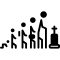
\includegraphics{./images/Leef}

\end{column}

\begin{column}{0.34\textwidth}

~

\end{column}

\begin{column}{0.33\textwidth}

\textbf{Leef} \citep{Leef} {[}\emph{Żyj}{]} to piosenka o życiu i umieraniu. Rozpoczyna się w scenerii podobnej do tej z piosenki wykonanej przez ojca André Hazes \ref{Een-beetje-verliefd}.

\end{column}

\vfill

\begin{column}{0.48\textwidth}

Op een vrijdag in de kroeg ergens in Amsterdam\\
Zat aan de bar met een glas een oude wijze man\\
Hij zei dat die nog maar een paar dagen had\\
Dus pak het leven, pak alles en ga er mee op pad

\end{column}

\begin{column}{0.04\textwidth}

~

\end{column}

\begin{column}{0.48\textwidth}

W piątek w pubie w Amsterdamie siedział\\
Stary mądry człowiek ze szklanką przy barze\\
Powiedział, że zostało mu jeszcze tylko kilka dni\\
Więc chwytaj życie, łap wszystko i ruszaj ze mną

\end{column}

\vfill

\begin{column}{0.48\textwidth}

\emph{En hij zei: '\,'Leef, alsof het je laatste dag is}\\
\emph{Leef, alsof de morgen niet bestaat}\\
\emph{Leef, alsof het nooit echt af is}\\
\emph{En leef, pak alles wat je kan'\,'}

\end{column}

\begin{column}{0.04\textwidth}

~

\end{column}

\begin{column}{0.48\textwidth}

\emph{I rzekł: '\,'Żyj, jakby to był twój ostatni dzień}\\
\emph{Żyj, jakby nie miało być jutra}\\
\emph{Żyj, jakby to nie był koniec do końca}\\
\emph{I żyj, łap wszystko'\,'}

\end{column}

\vfill

\begin{column}{0.48\textwidth}

\emph{En ga, a, a, a}\\
\emph{A, a, a, a}\\
\emph{A, a, a, a}\\
\emph{Pak alles wat je kan}

\end{column}

\begin{column}{0.04\textwidth}

~

\end{column}

\begin{column}{0.48\textwidth}

\emph{I leć, a, a, a}\\
\emph{A, a, a, a}\\
\emph{A, a, a, a}\\
\emph{Łap wszystko, co możesz}

\end{column}

\vfill

\begin{column}{0.48\textwidth}

\emph{En ga, a, a, a}\\
\emph{A, a, a, a}\\
\emph{Ga}\\
\emph{Pak alles wat je kan}

\end{column}

\begin{column}{0.04\textwidth}

~

\end{column}

\begin{column}{0.48\textwidth}

\emph{I leć, a, a, a}\\
\emph{A, a, a, a}\\
\emph{Leć}\\
\emph{Łap wszystko, co możesz}

\end{column}

\vfill

\begin{column}{0.48\textwidth}

Hij vertelde dat 'ie zich had gewerkt in het zweet\\
Geld verdiend als water maar nooit echt had geleefd\\
Z'n vrouw was bij hem weg, voor een ander ingeruild\\
Af en toe gelachen maar veel te veel gehuild

\end{column}

\begin{column}{0.04\textwidth}

~

\end{column}

\begin{column}{0.48\textwidth}

Opowiedział, jak się w życiu napocił przy robocie\\
Pieniądze spływały lekko ale nigdy nie żył naprawdę\\
Żona go opuściła zamieniła sobie na innego\\
Zbyt mało śmiał się a zbyt dużo się napłakał

\end{column}

\vfill

\begin{quote}
\textbf{Hij is zo vlug als water.} On chwyta w biegu.\\
\textbf{Ik wilde net op pad gaan.} Właśnie miałem wyruszyć w drogę.\\
\textbf{Gele gans zelf.} Zażółć gęślą jaźń.
\end{quote}

\hypertarget{Een-beetje-verliefd}{%
\section{\texorpdfstring{Een beetje verliefd, \emph{André Hazes}}{Een beetje verliefd, André Hazes}}\label{Een-beetje-verliefd}}

\begin{column}{0.33\textwidth}

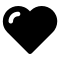
\includegraphics{./images/Een-beetje-verliefd}

\end{column}

\begin{column}{0.34\textwidth}

~

\end{column}

\begin{column}{0.33\textwidth}

\textbf{Een beetje verliefd} \citep{Een-beetje-verliefd} {[}\emph{Trochę zakochany}{]} to piosenka o niespełnionej miłości Rozpoczyna się w scenerii podobnej do tej z piosenki wykonanej przez syna André Hazes jr. \ref{Leef}.

\end{column}

\vfill

\begin{column}{0.48\textwidth}

In een discotheek, zat ik van de week\\
En ik voelde mij daar zo alleen\\
't Was er warm en druk, ik zat naast een lege kruk\\
Ik verlangde zo naar jou hier aan m'n zij

\end{column}

\begin{column}{0.04\textwidth}

~

\end{column}

\begin{column}{0.48\textwidth}

W jakiejś dyskotece byłem na tygodniu\\
I czułem się tam bardzo samotny\\
Było tam gorąco i tłoczno, siedziałem przy pustym stołku\\
Tak pragnąłem cię tutaj przy moim boku

\end{column}

\vfill

\begin{column}{0.48\textwidth}

Ja, ik denk nog steeds hoe het was geweest\\
Toen je naast me zat hier aan de bar\\
Ik vroeg: `'Drink je mee?'', dat vond jij oké\\
Toen je proostend naar me keek werd ik zo week

\end{column}

\begin{column}{0.04\textwidth}

~

\end{column}

\begin{column}{0.48\textwidth}

Tak, wciąż się zastanawiam, jak to było\\
Gdy się do mnie przysiadłaś przy barze\\
Spytałem: `'Napijesz się ze mną?'', zgodziłaś się\\
Kiedy na mnie spojrzałaś przy toaście, stałem się taki miękki

\end{column}

\vfill

\begin{column}{0.48\textwidth}

\emph{Een beetje verliefd, ik dacht een beetje verliefd}\\
\emph{Als ik wist wat jij toen dacht, had ik nooit op jou gewacht}\\
\emph{Als een kind zat ik te dromen deze nacht ben jij voor mij}\\
\emph{Maar die droom ging snel voorbij}

\end{column}

\begin{column}{0.04\textwidth}

~

\end{column}

\begin{column}{0.48\textwidth}

\emph{Trochę zakochany, myślałem trochę zakochany}\\
\emph{Gdybym wiedział, co wtedy myślisz, nigdy bym na ciebie nie czekał}\\
\emph{Jak małe dziecko ciągle marzyłem, tej nocy jesteś dla mnie}\\
\emph{Ale ten sen szybko minął}

\end{column}

\vfill

\begin{column}{0.48\textwidth}

Jij stond op en zei: `'Hou m'n plaatsje vrij\\
Ik moet even weg maar ben zo terug''\\
Ach, die kruk bleef leeg tot ik in de gaten kreeg\\
Dat je wegging zonder mij, ik was nu alleen

\end{column}

\begin{column}{0.04\textwidth}

~

\end{column}

\begin{column}{0.48\textwidth}

Wstałaś i powiedziałaś: `'Zajmij mi miejsce\\
Muszę na chwilę wyjść, ale zaraz wrócę''\\
Ach, ten stołek stał pusty, dopóki nie zauważyłem\\
Że odeszłaś beze mnie, teraz byłem sam

\end{column}

\vfill

\begin{quote}
\textbf{Weet je wat, ik ben er zat van.} Wiesz co, mam tego dosyć.\\
\textbf{Ik verlang ernaar met je alleen te zijn.} Pragnę być z tobą sam.\\
\textbf{Ik heb de wet aan m'n zij(-de).} Prawo mam po swojej stronie.\\
\textbf{Dat vind ik erg leuk.} To mi się bardzo podoba.\\
\textbf{We zitten te praten.} Gadamy sobie.\\
\textbf{Ik krijg dit in de gaten.} Zdaję sobie sprawę z tego
\end{quote}

\hypertarget{lata-1980---1989}{%
\chapter{Lata 1980 - 1989}\label{lata-1980---1989}}

Miejsce na rozdział

\hypertarget{lata-1990---1999}{%
\chapter{Lata 1990 - 1999}\label{lata-1990---1999}}

Miejsce na rozdział

\hypertarget{lata-2000---2009}{%
\chapter{Lata 2000 - 2009}\label{lata-2000---2009}}

Miejsce na rozdział

\hypertarget{lata-2010---2019}{%
\chapter{Lata 2010 - 2019}\label{lata-2010---2019}}

Miejsce na rodział

  \bibliography{songs.bib}

\end{document}
